\chapter{Contexte général de l'étude}

\section*{Introduction}
Ce stage resulte de plusieurs collaborations. D’une part elle result d’une collabo-
ration entre l’Université Nazi Bonin et L’université Lumière Lyon 2 dans le cadre du
programme erasmus+ mobilité etudiantes. C’est dans ce cadre que nous avons été
acceuillit au dans les locaux du LIRIS au sein de l’Université Lumière Lyon 2. Ce su-
jet de stage intitulé «segmentation géométrique et ghotométrique d’images acquises
par drones», resulte aussi d’une collaboration entre la société TECNI DRONE basée
à Baix (Ardèche) et l’equipe Imagine du LIRIS (site de l’Université Lumière Lyon
2 à Bron). TECNI DRONE se specialise dans la formation de pilot de drones et dans
l’acquisition de données géométriques issues de mines et de carrières. Les campagnes
d’acquisition d’images par drones, en milieu naturel, permettent de produire avec un
très haut niveau de qualité, des modèles numériques de terrains texturés, porteurs à
la fois d’informations géométriques et d’informations photométriques extrêmement
riches. De nombreuses recherches ont été menées au cours des dernières années, pour
affiner la qualité du traitement de ces données visuelles, et produire des maillages
texturés de plus en plus fiables. En revanche, l’exploitation de ces données reste pour
l’instant limitée soit à des traitements géométriques effectués sur les maillages 3D,
soit à des traitements d’images 2D, effectués par exemple sur les ortho-images obtenues 
par assemblage des multiples vues partielles.

\section{La structure d'accueil}

\subsection{Présentation }

 \subsubsection{Présentation du LIRIS}

Nous avons effectué notre stage au sein du Laboratoire d'InfoRmatique en 
Image et Systeme d'information \nomenclature{LIRIS}{Laboratoire d'InfoRmatique en Image et Systeme d'information}.
Le \nomenclature{LIRIS}{Laboratoire d'InfoRmatique en Image et Systeme d'information}est une unité miste de recherche  (\nomenclature{UMR}{Unité Mixte de Recherche} 5205) porté par
\begin{itemize}
  \item le CNRS
  \item l'INSA de Lyon
  \item l'Université Claude Bernard Lyon 1
  \item l'Université Lumière Lyon 2
  \item l'Ecole Centrale de Lyon
\end{itemize}
Il compte 330 membres, et a pour principal champ scientifique 
l'Informatique et plus généralement les Sciences et Technologies de l’Information.
Une partie importante de la recherche effectuée au LIRIS s’étend à la frontière de notre 
discipline, au service de problématiques sociétales importantes. Certaines des ses activités de 
recherche se situent aux interfaces de l’ingénierie, des sciences humaines et sociales, des sciences 
de la vie et des sciences de l’environnement. L’ensemble des 6 pôles de compétences du LIRIS participe 
de façon équilibrée à la valorisation des travaux de recherche. Par ailleurs, le LIRIS entretient de 
nombreuses relations avec son environnement social, économique et culturel, aussi bien aux niveaux 
local et régional qu’au niveau  national. 
Les interactions avec les entreprises s’établissent au travers de projets collaboratifs.
Le LIRIS couvre des thématiques scientifiques structurées en 6 pôles de compétences regroupant 14 équipes. 
\begin{itemize}
  \item Simulation, virtualité \& sciences computationnelles (Equipes Beagle, R3AM, SAARA)
  \item Géométrie \& modélisation (Equipes GeoMod, M2DisCo)
  \item Science des données (Equipes BD, DM2L, GOAL)
  \item Vision intelligente \& reconnaissance visuelle (Equipe Imagine)
  \item Interactions \& cognition (Equipes SICAL, SMA, TWEAK)
  \item Services, systèmes distribués, sécurité (Equipes DRIM, SOC)
\end{itemize}

Les travaux des équipes de recherche trouvent aussi des applications dans les secteurs : 
Biologie et santé (modelisation du vivant, ingénierie pour la santé), Intelligence ambiante 
(systèmes pervasifs et distribués, monitoring intelligent, systèmes autonomes), Apprentissage
humain (personnalisation, assistance cognitive, assistance à l'apprentissage collaboratif, 
jeux sérieux, loisirs numériques), Calcul scientifique (traitement de grandes masses de données
– big data).


\subsubsection{Presentation de l'equipe Imagine}
Nous avons effectués notre stage au sein de l'equipe Imagine sur le site de l'
université Lumière Lyon 2 à Bron.
L’équipe Imagine du LIRIS est spécialisée dans la vision par ordinateur, l’apprentissage 
et la reconnaissance de formes. Elle réunit 21 membres permanents (8 PR, 3 MCF-HDR et 10 MCF), 
enseignants-chercheurs de l’Université Lyon 1, de l’Université Lyon 2, de l’École Centrale de 
Lyon et de l’INSA Lyon.
En 2019, elle compte également parmi ses membres 29 doctorants et 17 post-doctorants.
Les différentes activités de recherche menées dans l’équipe Imagine partagent les mêmes 
objectifs généraux visant la compréhension d’images multi-sources et multi-capteurs, 
intégrant ainsi une très large variété de contenus autour des images de personnes, d’objets 
et de scènes en 2D et 3D (scènes naturelles ou urbaines, images aériennes et satellites, visages…), 
des séquences d’images et des flux vidéos, ainsi que des documents numérisés (cartes, textes écrits et 
imprimés, partitions et symboles…). La notion d’objet visuel, au sens large, constitue ainsi un 
dénominateur commun de nos recherches.
Les activités de l’équipe Imagine se déclinent en différentes thématiques 
liées à la mise en œuvre de méthodes d’indexation, de modélisation, 
de classification et de reconnaissance du contenu (objets, actions, concepts), 
avec une attention particulière portée au développement de méthodes d’apprentissage 
automatique pour la vision par ordinateur.
Les recherches menées dans l’équipe Imagine visent à construire des passerelles pour 
franchir le fossé sémantique entre, d’une part, les informations de bas niveau présentes 
dans les données brutes (données échantillonnées issues du signal), les éventuelles données 
multi-sources issues d’autres modalités ou capteurs (cas notamment des applications embarquées) 
et les informations de plus haut niveau sémantique qui reposent sur la modélisation, la 
classification et l’identification des contenus.
L’activité de recherche de l’équipe Imagine relève de 5 
sous-thèmes majeurs qui constituent le cœur de ses applications.

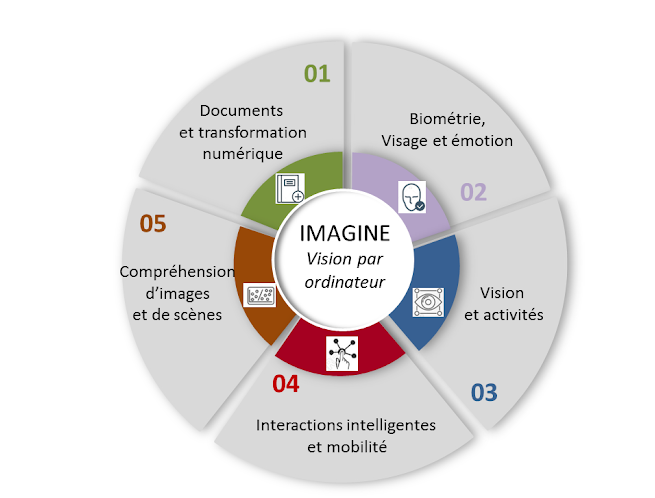
\includegraphics[scale=0.4]{images/Imagine.png}~\\[0.8cm]


 

  \subsection{Organisation}
   \subsubsection{Organigramme}  
L'organnigramme du LIRIS se présente comme suit: 
(voir Figure \ref{fig:organigramme}).
 \begin{figure}[h!]
  \begin{center}
    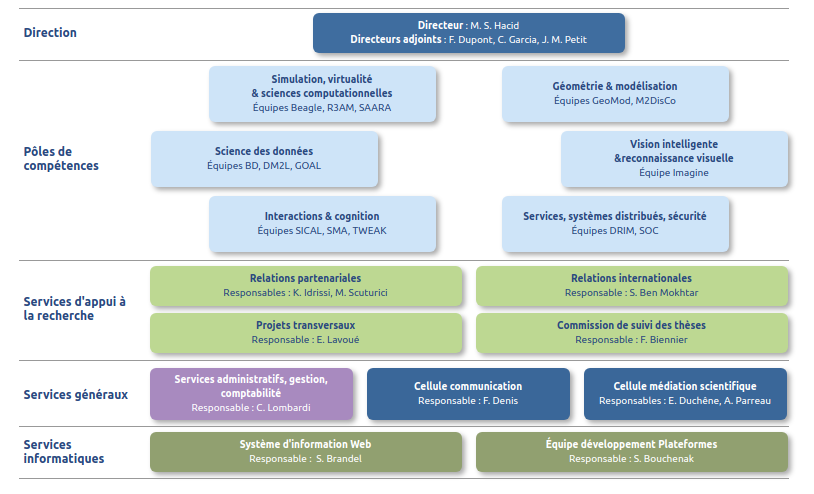
\includegraphics[width=17cm]{images/OrganigrammeLiris.png}
\caption{Organigramme du LIRIS.\label{fig:organigramme}}
\end{center}
\end{figure}


 \section{Présentation du sujet}

\subsection{Intitulé de sujet}

\textbf{Segmentation Géométrique etPhotométrique d’images Acquises par Drones}

 \subsection{Contexte du sujet}



\subsection{Intérêt du sujet}
 
Ce projet est très important pour Technidrone dans la mesure ou elle vise à
assister les techniciens de Technidrone dans leur tache d'annotation par la meme occasions reduire de façon 
significative le temps de travail de ces derniers.
Les résultats attendus sont:
\begin{itemize}
  \item Un gain en temps;
  \item Identification automatique des formes geometriques dans les images;
  \item 
\end{itemize}

    \subsection{Problématique du sujet}

    L’exploitation de données recoltées lors des campagnes d'acquisition reste pour
    l’instant limitée soit à des traitements géométriques effectués sur les maillages 3D,
    soit à des traitements d’images 2D, effectués par exemple sur les ortho-images obtenues
    par assemblage des multiples vues partielles. En revanche, la qualification de
    ces données, indispensable aux exploitants, reste pour l’instant un travail essentiellement manuel.
    Il s’agit par exemple, d’identifier les ruptures de pentes qui délimitent
    les voies de roulement des engins, de calculer la largeur de ces voies, de délimiter
    les hauts et les bas de talus, de calculer le volume des tas correspondant aux matériaux 
    extraits des carrières, etc. Ce processus qui est très important pour créer la
    carte d’une mine ou d’une carrière prend une dizaine d’heures pour un personnel
    entraîné. Une première etude effectuée au sein du laboratoire, axée essentiellement
    sur la geometrie contenue dans les maillages 3D a permis d’obtenir 62\% de rappel
    et 10\% de precision.

\subsection{Objectifs}

L’objectif de stage est d’utiliser d'une part les informations issues de la texture pour 
ameliorer les resultats obtenus en se basant uniquement sur la geometrie, et d'autre part, d’utiliser
de manière conjointe des informations issues des maillages, 
décrivant la géométrie de la scène, avec des données issues de la texture, portant des informations 
sur les discontinuités photométriques du terrain, pour assister les opérateurs dans leur tâche d’annotation 
des modèles numériques, construits à partir des images acquises par les drones.
En se basant sur des terrains déjà annotés, et en entraînant des classifieurs à reconnaître
les structures géométriques ou les motifs d’intérêt, nous voulons évaluer la capacité d’un système automatisé 
à effectuer cette identification avec un taux de succès le plus élevé possible. La tâche de 
l’opérateur se limiterait alors à la correction des inévitables erreurs de classification.

\section{Traitement des données et formats de fichiers}

TECHNI DRONE utilise plusieurs logiciels pour le traitement des donnéées après
les campagnes d'acquisition faites par drones. Cette etape est tres importante 
dans la mesure ou elle aboutie à la realisation des carte representant une carriere.

\begin{figure}[h]
  \begin{minipage}[c]{.46\linewidth}
      \centering
      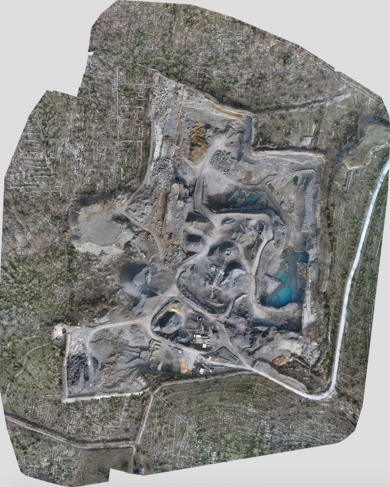
\includegraphics[width=8cm, height=8cm]{images/orthomosaique.png}
  \end{minipage}
  \hfill%
  \begin{minipage}[c]{.46\linewidth}
      \centering
      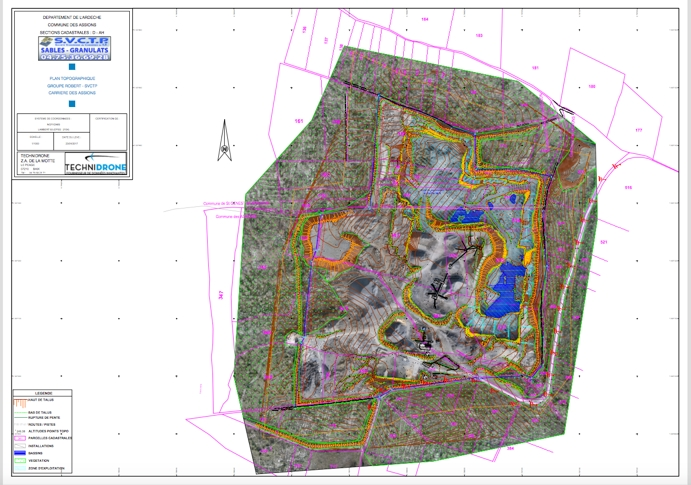
\includegraphics[width=8cm,height=8cm]{images/carteCarriere.jpg}
  \end{minipage}
  \caption{L’ortho mosaïque de la carrière et la carte de la carrière.
     \label{fig:credit}}
\end{figure}

\subsection{Pix4D}

Le traitement des images acquisent par drones est fait avec le logiciel Pix4D.
Pix4D est un logiciel de photogrammétrie pour la cartographie professionnelle 
basée sur des images de drones uniquement. 
\begin{figure}[h]
  \begin{center}
    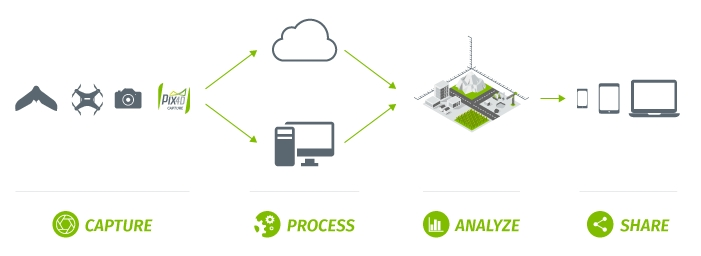
\includegraphics[width=12cm]{images/processusPix4D.jpg}
     \caption{Processus de traitement Pix4D.
     \label{ProcesPix4D}}
  \end{center}
\end{figure}
Le logiciel convertit les images 
aeriennes prise par drones en orthomosaiques 2D georeferencées, en model 
surface 3D texturé et en nuages de points. ce processus prend environ une dizaine
d'heures comment le montre la Figure~\ref{ProcesPix4D}. 

Dans la Figure~\ref{positionImage}, les points rouges representent les positions
des images prises drone et Les croix bleues sont les points GCPs
(Group Control Point)\footnote{Les GPCs sont des 
marqueurs visuels sur le sol avec des coordonnées connues qui augmentent 
la précision ortho mosaïque et permettent l'alignement de plusieurs 
campagnes d’acquisition.}. Le logiciel utilise les coordonnées des ces point
pour faire le recalage des images et produit les nuages de point et le maillage 3D
de la carrière. Le logiciel met aussi à disposition des outiles pour la detection
manuel des ligne de ruptures de pente directement sur les nuages de points ou
sur le maillage 3D. Les coordonnées de ces ligne ainsi detecter sont enregistrer
dans un fichier au format shapefile(.shp)\footnote{Shapefile est un format
de fichier ouvert compatible avec le logiciel OpenSource QGIS}. Cette phase
d'annotation prend egalement une dizaine d'heure pour un employé habitué au logiciel.
La Figure~\ref{annotationMallage} montre triangulaire 3D créé par pix4D,
sur lequel se basé pour détecter les lignes de ruptures de pente.

\begin{figure}[h]
  \begin{center}
    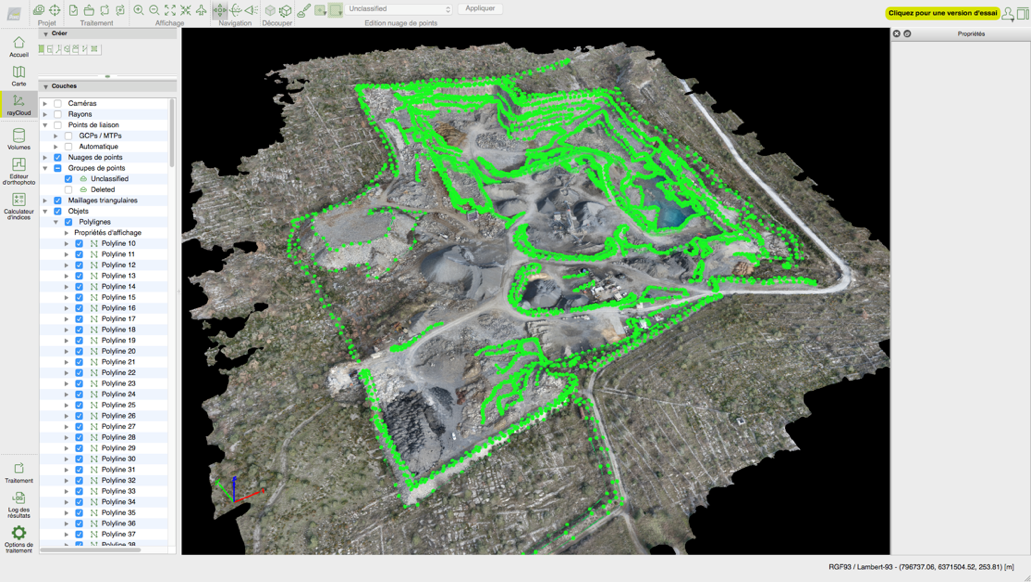
\includegraphics[width=12cm, height=5cm]{images/detctionLigne.jpg}
     \caption{Detection manuel des lignes de ruptures de pente.
     \label{detctionLigne}}
  \end{center}
\end{figure}
\begin{figure}[h]
  \begin{center}
    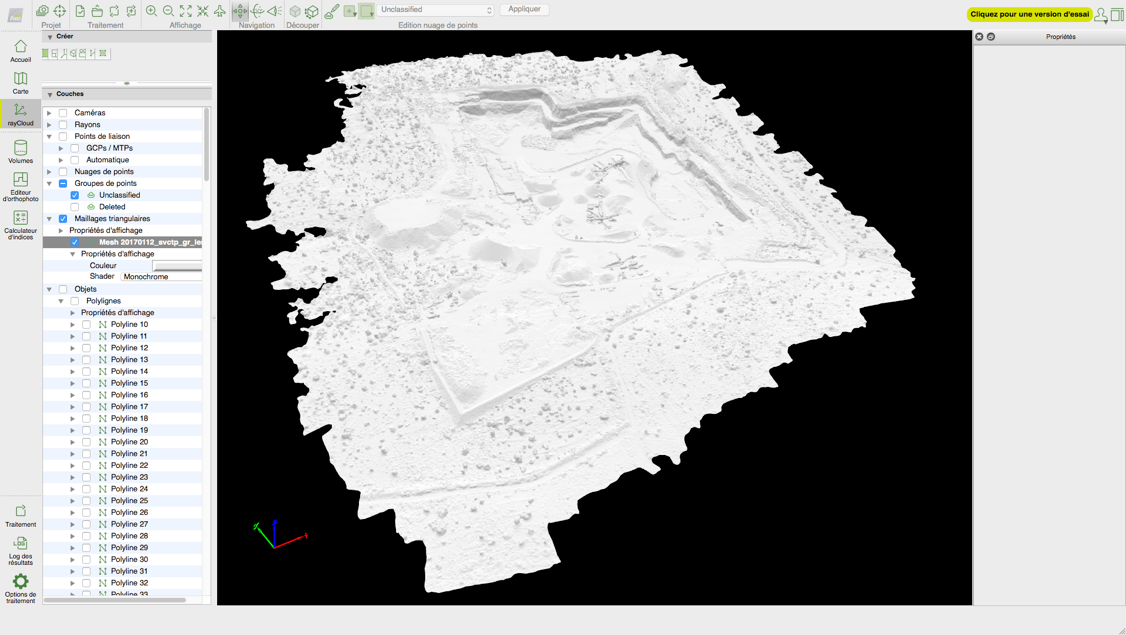
\includegraphics[width=12cm,height=5cm]{images/maillageSansTexture.jpg}
     \caption{Maillage 3D sans texture.
     \label{maillageSansTexture}}
  \end{center}
\end{figure}
\begin{figure}[h]
  \begin{center}
    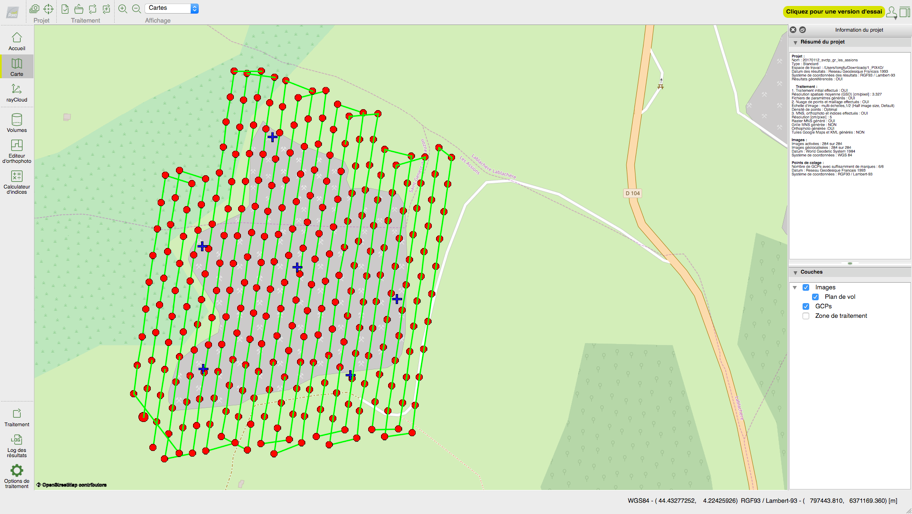
\includegraphics[width=12cm]{images/positionImagePix4D.jpg}
     \caption{Position des images prise par drones.
     \label{positionImage}}
  \end{center}
\end{figure}

\subsection{QGIS}

QGIS est un logiciel SIG (système d'information 
géographique) libre multiplate-forme publié sous licence GPL. 
il gère les formats d’image matricielles (raster) et vectorielles,
ainsi que les bases de données [Wikipedia](https://en.wikipedia.org/wiki/)\dots
TECHNI-DRONE utilise ce logiciel pour classifier les lignes de 
ruptures de pente par rapport aux courbes de niveau.
\begin{figure}[h]
  \begin{center}
    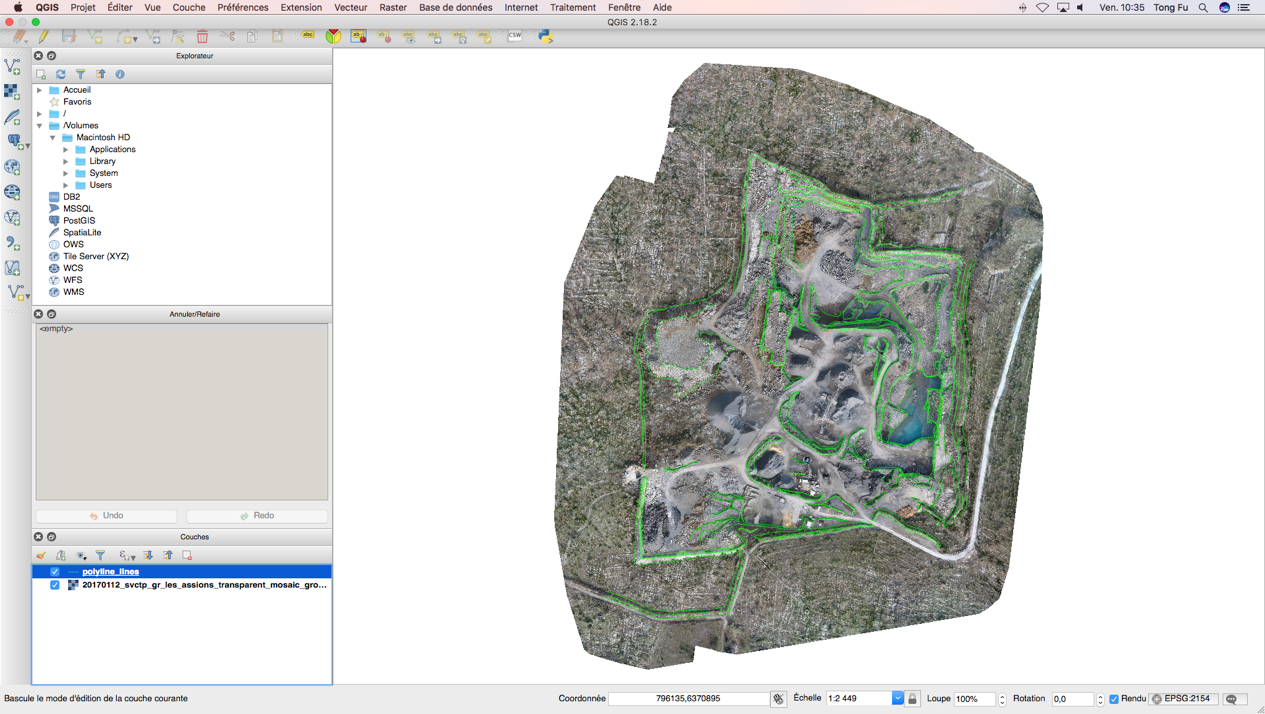
\includegraphics[width=12cm]{images/QGIS.jpg}
     \caption{Classification sur QGIS.
     \label{QGISClassification}}
  \end{center}
\end{figure}


\section*{Conclusion}
Dans ce chapitre il  a été question dans ce chapitre de présenter  la structure d’accueil,
au sein de laquelle nous avons menés nos travaux de recherche. .Ensuite nous avons
présenté le sujet qui qui fait objet de ce memoire, dégager sa problématique et
l’intérêt qu’il suscite pour la Société Technidrone. Dans le chapitre suivant,
nous parlerons des techniques machine learning, de la segmentation et de la classification.
